% -------------------------------------------------------------------------
% ------ nuweb macros (redefine as desired, or omit with "nuweb -p") ------
% -------------------------------------------------------------------------
\providecommand{\NWtxtMacroDefBy}{Macro defined by}
\providecommand{\NWtxtMacroRefIn}{Macro referenced in}
\providecommand{\NWtxtMacroNoRef}{Macro never referenced}
\providecommand{\NWtxtDefBy}{Defined by}
\providecommand{\NWtxtRefIn}{Referenced in}
\providecommand{\NWtxtNoRef}{Not referenced}
\providecommand{\NWtxtFileDefBy}{File defined by}
\providecommand{\NWsep}{${\diamond}$}
\providecommand{\NWlink}[2]{\hyperlink{#1}{#2}}
\providecommand{\NWtarget}[2]{% move baseline up by \baselineskip 
  \raisebox{\baselineskip}[1.5ex][0ex]{%
    \mbox{%
      \hypertarget{#1}{%
        \raisebox{-1\baselineskip}[0ex][0ex]{%
          \mbox{#2}%
}}}}}
% -------------------------------------------------------------------------

\documentclass[11pt,oneside]{article}	%use"amsart"insteadof"article"forAMSLaTeXformat
\usepackage{geometry}		%Seegeometry.pdftolearnthelayoutoptions.Therearelots.
\geometry{letterpaper}		%...ora4paperora5paperor...
%\geometry{landscape}		%Activateforforrotatedpagegeometry
%\usepackage[parfill]{parskip}		%Activatetobeginparagraphswithanemptylineratherthananindent
\usepackage{graphicx}				%Usepdf,png,jpg,orepsßwithpdflatex;useepsinDVImode
								%TeXwillautomaticallyconverteps-->pdfinpdflatex		
\usepackage{amssymb}
\usepackage{hyperref}

%----macros begin---------------------------------------------------------------
\usepackage{color}
\usepackage{amsthm}

\def\conv{\mbox{\textrm{conv}\,}}
\def\aff{\mbox{\textrm{aff}\,}}
\def\E{\mathbb{E}}
\def\R{\mathbb{R}}
\def\Z{\mathbb{Z}}
\def\tex{\TeX}
\def\latex{\LaTeX}
\def\v#1{{\bf #1}}
\def\p#1{{\bf #1}}
\def\T#1{{\bf #1}}

\def\vet#1{{\left(\begin{array}{cccccccccccccccccccc}#1\end{array}\right)}}
\def\mat#1{{\left(\begin{array}{cccccccccccccccccccc}#1\end{array}\right)}}

\def\lin{\mbox{\rm lin}\,}
\def\aff{\mbox{\rm aff}\,}
\def\pos{\mbox{\rm pos}\,}
\def\cone{\mbox{\rm cone}\,}
\def\conv{\mbox{\rm conv}\,}
\newcommand{\homog}[0]{\mbox{\rm homog}\,}
\newcommand{\relint}[0]{\mbox{\rm relint}\,}

%----macros end-----------------------------------------------------------------

\title{Domain mapping with LAR
\footnote{This document is part of the \emph{Linear Algebraic Representation with CoChains} (LAR-CC) framework~\cite{cclar-proj:2013:00}. \today}
}
\author{Alberto Paoluzzi}
%\date{}							%Activatetodisplayagivendateornodate

\begin{document}
\maketitle
\nonstopmode

\begin{abstract}
In this module a first implementation (no optimisations) is done of the \texttt{LARMAP} operator, reproducing the behaviour of the plasm \texttt{MAP} primitive, but with better handling of the topology, including the sewing of decomposed (simplicial domains) about their possible sewing.
\end{abstract}

\tableofcontents

%===============================================================================
\section{Domain decomposition}
%===============================================================================

\paragraph{Standard and scaled decomposition of unit domain}

%-------------------------------------------------------------------------------
\begin{flushleft} \small
\begin{minipage}{\linewidth} \label{scrap1}
\protect\makebox[0ex][r]{\NWtarget{nuweb1}{\rule{0ex}{0ex}}\hspace{1em}}$\langle\,$Generate a simplicial decomposition ot the $[0,1]^d$ domain\nobreak\ {\footnotesize 1}$\,\rangle\equiv$
\vspace{-1ex}
\begin{list}{}{} \item
\mbox{}\verb@def larDomain(shape):@\\
\mbox{}\verb@   V,CV = larSimplexGrid(shape)@\\
\mbox{}\verb@   V = scalePoints(V, [1./d for d in shape])@\\
\mbox{}\verb@   return V,CV@\\
\mbox{}\verb@@\\
\mbox{}\verb@def larIntervals(shape):@\\
\mbox{}\verb@   def larIntervals0(size):@\\
\mbox{}\verb@      V,CV = larDomain(shape)@\\
\mbox{}\verb@      V = scalePoints(V, [scaleFactor for scaleFactor in size])@\\
\mbox{}\verb@      return V,CV@\\
\mbox{}\verb@   return larIntervals0@\\
\mbox{}\verb@@{\NWsep}
\end{list}
\vspace{-1ex}
\footnotesize\addtolength{\baselineskip}{-1ex}
\begin{list}{}{\setlength{\itemsep}{-\parsep}\setlength{\itemindent}{-\leftmargin}}
\item \NWtxtMacroRefIn\ \NWlink{nuweb13a}{13a}.
\end{list}
\end{minipage}\\[4ex]
\end{flushleft}
%-------------------------------------------------------------------------------

%===============================================================================
\section{Embedding via coordinate functions}
%===============================================================================

\subsection{Mapping domain vertices}
%-------------------------------------------------------------------------------
\begin{flushleft} \small \label{scrap2}
\protect\makebox[0ex][r]{\NWtarget{nuweb2a}{\rule{0ex}{0ex}}\hspace{1em}}$\langle\,$Primitive mapping function\nobreak\ {\footnotesize 2a}$\,\rangle\equiv$
\vspace{-1ex}
\begin{list}{}{} \item
\mbox{}\verb@def larMap(coordFuncs):@\\
\mbox{}\verb@   def larMap0(domain):@\\
\mbox{}\verb@      V,CV = domain@\\
\mbox{}\verb@      V = TRANS(CONS(coordFuncs)(V))  # plasm CONStruction@\\
\mbox{}\verb@      return V,CV@\\
\mbox{}\verb@   return larMap0@\\
\mbox{}\verb@@{\NWsep}
\end{list}
\vspace{-1ex}
\footnotesize\addtolength{\baselineskip}{-1ex}
\begin{list}{}{\setlength{\itemsep}{-\parsep}\setlength{\itemindent}{-\leftmargin}}
\item \NWtxtMacroRefIn\ \NWlink{nuweb13a}{13a}.
\end{list}
\end{flushleft}
%-------------------------------------------------------------------------------

\subsection{Identify close or coincident points}

%-------------------------------------------------------------------------------
\begin{flushleft} \small \label{scrap3}
\protect\makebox[0ex][r]{\NWtarget{nuweb2b}{\rule{0ex}{0ex}}\hspace{1em}}$\langle\,$Create a dictionary with key the point location\nobreak\ {\footnotesize 2b}$\,\rangle\equiv$
\vspace{-1ex}
\begin{list}{}{} \item
\mbox{}\verb@def checkModel(model):@\\
\mbox{}\verb@   V,CV = model; n = len(V)@\\
\mbox{}\verb@   vertDict = defaultdict(list)@\\
\mbox{}\verb@   for k,v in enumerate(V): vertDict[vcode(v)].append(k) @\\
\mbox{}\verb@   verts = (vertDict.values())@\\
\mbox{}\verb@   invertedindex = [None]*n@\\
\mbox{}\verb@   for k,value in enumerate(verts):@\\
\mbox{}\verb@      for i in value:@\\
\mbox{}\verb@         invertedindex[i]=value[0]  @\\
\mbox{}\verb@   CV = [[invertedindex[v] for v in cell] for cell in CV]@\\
\mbox{}\verb@   # filter out degenerate cells@\\
\mbox{}\verb@   CV = [list(set(cell)) for cell in CV if len(set(cell))==len(cell)]@\\
\mbox{}\verb@   return V, CV@\\
\mbox{}\verb@@{\NWsep}
\end{list}
\vspace{-1ex}
\footnotesize\addtolength{\baselineskip}{-1ex}
\begin{list}{}{\setlength{\itemsep}{-\parsep}\setlength{\itemindent}{-\leftmargin}}
\item \NWtxtMacroRefIn\ \NWlink{nuweb13a}{13a}.
\end{list}
\end{flushleft}
%-------------------------------------------------------------------------------


%===============================================================================
\section{Embedding/Projecting models}
%===============================================================================
%-------------------------------------------------------------------------------

In order apply 3D transformations to a two-dimensional LAR model, we must embed it in 3D space, by adding one more coordinate to its vertices. 

\paragraph{Embedding and projecting a geometric model}

This task is performed by the following function \texttt{larEmbed} with parameter $k$, that inserts its $d$-dimensional geometric argument in the $x_{d+1}, \ldots, x_{d+k}=0$ subspace.
A reverse transformation of projection, removing the last $k$ coordinate of vertices without changing the object topology, is performed by the function \texttt{larEmbed} with \emph{negative} integer parameter.


%-------------------------------------------------------------------------------
\begin{flushleft} \small \label{scrap4}
\protect\makebox[0ex][r]{\NWtarget{nuweb3a}{\rule{0ex}{0ex}}\hspace{1em}}$\langle\,$Embedding and projecting a geometric model\nobreak\ {\footnotesize 3a}$\,\rangle\equiv$
\vspace{-1ex}
\begin{list}{}{} \item
\mbox{}\verb@def larEmbed(k):@\\
\mbox{}\verb@   def larEmbed0(model):@\\
\mbox{}\verb@      V,CV = model@\\
\mbox{}\verb@      if k>0:@\\
\mbox{}\verb@         V = [v+[0.]*k for v in V] @\\
\mbox{}\verb@      elif k<0:@\\
\mbox{}\verb@         V = [v[:-k] for v in V] @\\
\mbox{}\verb@      return V,CV@\\
\mbox{}\verb@   return larEmbed0@\\
\mbox{}\verb@@{\NWsep}
\end{list}
\vspace{-1ex}
\footnotesize\addtolength{\baselineskip}{-1ex}
\begin{list}{}{\setlength{\itemsep}{-\parsep}\setlength{\itemindent}{-\leftmargin}}
\item \NWtxtMacroRefIn\ \NWlink{nuweb13a}{13a}.
\end{list}
\end{flushleft}
%-------------------------------------------------------------------------------


%-------------------------------------------------------------------------------
%===============================================================================
\section{Primitive objets}
%===============================================================================
%-------------------------------------------------------------------------------
\subsection{1D primitives}
%-------------------------------------------------------------------------------

\paragraph{Curved line}
%-------------------------------------------------------------------------------
\begin{flushleft} \small \label{scrap5}
\protect\makebox[0ex][r]{\NWtarget{nuweb3b}{\rule{0ex}{0ex}}\hspace{1em}}$\langle\,$aaaa\nobreak\ {\footnotesize 3b}$\,\rangle\equiv$
\vspace{-1ex}
\begin{list}{}{} \item
\mbox{}\verb@@\\
\mbox{}\verb@@\\
\mbox{}\verb@@{\NWsep}
\end{list}
\vspace{-1ex}
\footnotesize\addtolength{\baselineskip}{-1ex}
\begin{list}{}{\setlength{\itemsep}{-\parsep}\setlength{\itemindent}{-\leftmargin}}
\item {\NWtxtMacroNoRef}.
\end{list}
\end{flushleft}
%-------------------------------------------------------------------------------

\paragraph{Circle}
%-------------------------------------------------------------------------------
\begin{flushleft} \small \label{scrap6}
\protect\makebox[0ex][r]{\NWtarget{nuweb3c}{\rule{0ex}{0ex}}\hspace{1em}}$\langle\,$Circle centered in the origin\nobreak\ {\footnotesize 3c}$\,\rangle\equiv$
\vspace{-1ex}
\begin{list}{}{} \item
\mbox{}\verb@def larCircle(radius=1.):@\\
\mbox{}\verb@   def larCircle0(shape=36):@\\
\mbox{}\verb@      domain = larIntervals([shape])([2*PI])@\\
\mbox{}\verb@      V,CV = domain@\\
\mbox{}\verb@      x = lambda V : [radius*COS(p[0]) for p in V]@\\
\mbox{}\verb@      y = lambda V : [radius*SIN(p[0]) for p in V]@\\
\mbox{}\verb@      return larMap([x,y])(domain)@\\
\mbox{}\verb@   return larCircle0@\\
\mbox{}\verb@@{\NWsep}
\end{list}
\vspace{-1ex}
\footnotesize\addtolength{\baselineskip}{-1ex}
\begin{list}{}{\setlength{\itemsep}{-\parsep}\setlength{\itemindent}{-\leftmargin}}
\item \NWtxtMacroRefIn\ \NWlink{nuweb13a}{13a}.
\end{list}
\end{flushleft}
%-------------------------------------------------------------------------------
%-------------------------------------------------------------------------------
\subsection{2D primitives}
%-------------------------------------------------------------------------------

\paragraph{Disk}
-------------------------------------------------------------------------------
\begin{flushleft} \small \label{scrap7}
\protect\makebox[0ex][r]{\NWtarget{nuweb3d}{\rule{0ex}{0ex}}\hspace{1em}}$\langle\,$Disk centered in the origin\nobreak\ {\footnotesize 3d}$\,\rangle\equiv$
\vspace{-1ex}
\begin{list}{}{} \item
\mbox{}\verb@def larDisk(radius=1.):@\\
\mbox{}\verb@   def larDisk0(shape=[36,1]):@\\
\mbox{}\verb@      domain = larIntervals(shape)([2*PI,radius])@\\
\mbox{}\verb@      V,CV = domain@\\
\mbox{}\verb@      x = lambda V : [p[1]*COS(p[0]) for p in V]@\\
\mbox{}\verb@      y = lambda V : [p[1]*SIN(p[0]) for p in V]@\\
\mbox{}\verb@      return larMap([x,y])(domain)@\\
\mbox{}\verb@   return larDisk0@\\
\mbox{}\verb@@{\NWsep}
\end{list}
\vspace{-1ex}
\footnotesize\addtolength{\baselineskip}{-1ex}
\begin{list}{}{\setlength{\itemsep}{-\parsep}\setlength{\itemindent}{-\leftmargin}}
\item \NWtxtMacroRefIn\ \NWlink{nuweb13a}{13a}.
\end{list}
\end{flushleft}
%-------------------------------------------------------------------------------

\paragraph{Ring}
-------------------------------------------------------------------------------
\begin{flushleft} \small \label{scrap8}
\protect\makebox[0ex][r]{\NWtarget{nuweb4a}{\rule{0ex}{0ex}}\hspace{1em}}$\langle\,$Ring centered in the origin\nobreak\ {\footnotesize 4a}$\,\rangle\equiv$
\vspace{-1ex}
\begin{list}{}{} \item
\mbox{}\verb@def larRing(params):@\\
\mbox{}\verb@   r1,r2 = params@\\
\mbox{}\verb@   def larRing0(shape=[36,1]):@\\
\mbox{}\verb@      V,CV = larIntervals(shape)([2*PI,r2-r1])@\\
\mbox{}\verb@      V = translatePoints(V,[0,r1])@\\
\mbox{}\verb@      domain = V,CV@\\
\mbox{}\verb@      x = lambda V : [p[1] * COS(p[0]) for p in V]@\\
\mbox{}\verb@      y = lambda V : [p[1] * SIN(p[0]) for p in V]@\\
\mbox{}\verb@      return larMap([x,y])(domain)@\\
\mbox{}\verb@   return larRing0@\\
\mbox{}\verb@@{\NWsep}
\end{list}
\vspace{-1ex}
\footnotesize\addtolength{\baselineskip}{-1ex}
\begin{list}{}{\setlength{\itemsep}{-\parsep}\setlength{\itemindent}{-\leftmargin}}
\item \NWtxtMacroRefIn\ \NWlink{nuweb13a}{13a}.
\end{list}
\end{flushleft}
%-------------------------------------------------------------------------------
\paragraph{Cylinder surface}
%-------------------------------------------------------------------------------
\begin{flushleft} \small \label{scrap9}
\protect\makebox[0ex][r]{\NWtarget{nuweb4b}{\rule{0ex}{0ex}}\hspace{1em}}$\langle\,$Cylinder surface with $z$ axis\nobreak\ {\footnotesize 4b}$\,\rangle\equiv$
\vspace{-1ex}
\begin{list}{}{} \item
\mbox{}\verb@from scipy.linalg import det@\\
\mbox{}\verb@"""@\\
\mbox{}\verb@def makeOriented(model):@\\
\mbox{}\verb@   V,CV = model@\\
\mbox{}\verb@   out = []@\\
\mbox{}\verb@   for cell in CV: @\\
\mbox{}\verb@      mat = scipy.array([V[v]+[1] for v in cell]+[[0,0,0,1]])@\\
\mbox{}\verb@      if det(mat) < 0.0:@\\
\mbox{}\verb@         out.append(cell)@\\
\mbox{}\verb@      else:@\\
\mbox{}\verb@         out.append([cell[1]]+[cell[0]]+cell[2:])@\\
\mbox{}\verb@      print "\n det(mat) =",det(mat)@\\
\mbox{}\verb@   return V,out@\\
\mbox{}\verb@"""@\\
\mbox{}\verb@def larCylinder(params):@\\
\mbox{}\verb@   radius,height= params@\\
\mbox{}\verb@   def larCylinder0(shape=[36,1]):@\\
\mbox{}\verb@      domain = larIntervals(shape)([2*PI,1])@\\
\mbox{}\verb@      V,CV = domain@\\
\mbox{}\verb@      x = lambda V : [radius*COS(p[0]) for p in V]@\\
\mbox{}\verb@      y = lambda V : [radius*SIN(p[0]) for p in V]@\\
\mbox{}\verb@      z = lambda V : [height*p[1] for p in V]@\\
\mbox{}\verb@      mapping = [x,y,z]@\\
\mbox{}\verb@      model = larMap(mapping)(domain)@\\
\mbox{}\verb@      # model = makeOriented(model)@\\
\mbox{}\verb@      return model@\\
\mbox{}\verb@   return larCylinder0@\\
\mbox{}\verb@@{\NWsep}
\end{list}
\vspace{-1ex}
\footnotesize\addtolength{\baselineskip}{-1ex}
\begin{list}{}{\setlength{\itemsep}{-\parsep}\setlength{\itemindent}{-\leftmargin}}
\item \NWtxtMacroRefIn\ \NWlink{nuweb13a}{13a}.
\end{list}
\end{flushleft}
%-------------------------------------------------------------------------------
\paragraph{Spherical surface of given radius}
%-------------------------------------------------------------------------------
\begin{flushleft} \small \label{scrap10}
\protect\makebox[0ex][r]{\NWtarget{nuweb5a}{\rule{0ex}{0ex}}\hspace{1em}}$\langle\,$Spherical surface of given radius\nobreak\ {\footnotesize 5a}$\,\rangle\equiv$
\vspace{-1ex}
\begin{list}{}{} \item
\mbox{}\verb@def larSphere(radius=1):@\\
\mbox{}\verb@   def larSphere0(shape=[18,36]):@\\
\mbox{}\verb@      V,CV = larIntervals(shape)([PI,2*PI])@\\
\mbox{}\verb@      V = translatePoints(V,[-PI/2,-PI])@\\
\mbox{}\verb@      domain = V,CV@\\
\mbox{}\verb@      x = lambda V : [radius*COS(p[0])*COS(p[1]) for p in V]@\\
\mbox{}\verb@      y = lambda V : [radius*COS(p[0])*SIN(p[1]) for p in V]@\\
\mbox{}\verb@      z = lambda V : [radius*SIN(p[0]) for p in V]@\\
\mbox{}\verb@      return larMap([x,y,z])(domain)@\\
\mbox{}\verb@   return larSphere0@\\
\mbox{}\verb@@{\NWsep}
\end{list}
\vspace{-1ex}
\footnotesize\addtolength{\baselineskip}{-1ex}
\begin{list}{}{\setlength{\itemsep}{-\parsep}\setlength{\itemindent}{-\leftmargin}}
\item \NWtxtMacroRefIn\ \NWlink{nuweb13a}{13a}.
\end{list}
\end{flushleft}
%-------------------------------------------------------------------------------
\paragraph{Toroidal surface}
%-------------------------------------------------------------------------------
\begin{flushleft} \small \label{scrap11}
\protect\makebox[0ex][r]{\NWtarget{nuweb5b}{\rule{0ex}{0ex}}\hspace{1em}}$\langle\,$Toroidal surface of given radiuses\nobreak\ {\footnotesize 5b}$\,\rangle\equiv$
\vspace{-1ex}
\begin{list}{}{} \item
\mbox{}\verb@def larToroidal(params):@\\
\mbox{}\verb@   r,R = params@\\
\mbox{}\verb@   def larToroidal0(shape=[24,36]):@\\
\mbox{}\verb@      domain = larIntervals(shape)([2*PI,2*PI])@\\
\mbox{}\verb@      V,CV = domain@\\
\mbox{}\verb@      x = lambda V : [(R + r*COS(p[0])) * COS(p[1]) for p in V]@\\
\mbox{}\verb@      y = lambda V : [(R + r*COS(p[0])) * SIN(p[1]) for p in V]@\\
\mbox{}\verb@      z = lambda V : [-r * SIN(p[0]) for p in V]@\\
\mbox{}\verb@      return larMap([x,y,z])(domain)@\\
\mbox{}\verb@   return larToroidal0@\\
\mbox{}\verb@@{\NWsep}
\end{list}
\vspace{-1ex}
\footnotesize\addtolength{\baselineskip}{-1ex}
\begin{list}{}{\setlength{\itemsep}{-\parsep}\setlength{\itemindent}{-\leftmargin}}
\item \NWtxtMacroRefIn\ \NWlink{nuweb13a}{13a}.
\end{list}
\end{flushleft}
%-------------------------------------------------------------------------------
\paragraph{Crown surface}
%-------------------------------------------------------------------------------
\begin{flushleft} \small \label{scrap12}
\protect\makebox[0ex][r]{\NWtarget{nuweb6a}{\rule{0ex}{0ex}}\hspace{1em}}$\langle\,$Half-toroidal surface of given radiuses\nobreak\ {\footnotesize 6a}$\,\rangle\equiv$
\vspace{-1ex}
\begin{list}{}{} \item
\mbox{}\verb@def larCrown(params):@\\
\mbox{}\verb@   r,R = params@\\
\mbox{}\verb@   def larCrown0(shape=[24,36]):@\\
\mbox{}\verb@      V,CV = larIntervals(shape)([PI,2*PI])@\\
\mbox{}\verb@      V = translatePoints(V,[-PI/2,0])@\\
\mbox{}\verb@      domain = V,CV@\\
\mbox{}\verb@      x = lambda V : [(R + r*COS(p[0])) * COS(p[1]) for p in V]@\\
\mbox{}\verb@      y = lambda V : [(R + r*COS(p[0])) * SIN(p[1]) for p in V]@\\
\mbox{}\verb@      z = lambda V : [-r * SIN(p[0]) for p in V]@\\
\mbox{}\verb@      return larMap([x,y,z])(domain)@\\
\mbox{}\verb@   return larCrown0@\\
\mbox{}\verb@@{\NWsep}
\end{list}
\vspace{-1ex}
\footnotesize\addtolength{\baselineskip}{-1ex}
\begin{list}{}{\setlength{\itemsep}{-\parsep}\setlength{\itemindent}{-\leftmargin}}
\item \NWtxtMacroRefIn\ \NWlink{nuweb13a}{13a}.
\end{list}
\end{flushleft}
%-------------------------------------------------------------------------------

%-------------------------------------------------------------------------------
\subsection{3D primitives}
%-------------------------------------------------------------------------------

\paragraph{Ball}
%-------------------------------------------------------------------------------
\begin{flushleft} \small \label{scrap13}
\protect\makebox[0ex][r]{\NWtarget{nuweb6b}{\rule{0ex}{0ex}}\hspace{1em}}$\langle\,$Solid Sphere of given radius\nobreak\ {\footnotesize 6b}$\,\rangle\equiv$
\vspace{-1ex}
\begin{list}{}{} \item
\mbox{}\verb@def larBall(radius=1):@\\
\mbox{}\verb@   def larBall0(shape=[18,36]):@\\
\mbox{}\verb@      V,CV = checkModel(larSphere(radius)(shape))@\\
\mbox{}\verb@      return V,[range(len(V))]@\\
\mbox{}\verb@   return larBall0@\\
\mbox{}\verb@@{\NWsep}
\end{list}
\vspace{-1ex}
\footnotesize\addtolength{\baselineskip}{-1ex}
\begin{list}{}{\setlength{\itemsep}{-\parsep}\setlength{\itemindent}{-\leftmargin}}
\item \NWtxtMacroRefIn\ \NWlink{nuweb13a}{13a}.
\end{list}
\end{flushleft}
%-------------------------------------------------------------------------------

\paragraph{Solid cylinder}
%-------------------------------------------------------------------------------
\begin{flushleft} \small \label{scrap14}
\protect\makebox[0ex][r]{\NWtarget{nuweb6c}{\rule{0ex}{0ex}}\hspace{1em}}$\langle\,$Solid cylinder of given radius and height\nobreak\ {\footnotesize 6c}$\,\rangle\equiv$
\vspace{-1ex}
\begin{list}{}{} \item
\mbox{}\verb@def larRod(params):@\\
\mbox{}\verb@   radius,height= params@\\
\mbox{}\verb@   def larRod0(shape=[36,1]):@\\
\mbox{}\verb@      V,CV = checkModel(larCylinder(params)(shape))@\\
\mbox{}\verb@      return V,[range(len(V))]@\\
\mbox{}\verb@   return larRod0@\\
\mbox{}\verb@@{\NWsep}
\end{list}
\vspace{-1ex}
\footnotesize\addtolength{\baselineskip}{-1ex}
\begin{list}{}{\setlength{\itemsep}{-\parsep}\setlength{\itemindent}{-\leftmargin}}
\item \NWtxtMacroRefIn\ \NWlink{nuweb13a}{13a}.
\end{list}
\end{flushleft}
%-------------------------------------------------------------------------------

\paragraph{Solid torus}
%-------------------------------------------------------------------------------
\begin{flushleft} \small \label{scrap15}
\protect\makebox[0ex][r]{\NWtarget{nuweb7a}{\rule{0ex}{0ex}}\hspace{1em}}$\langle\,$Solid torus of given radiuses\nobreak\ {\footnotesize 7a}$\,\rangle\equiv$
\vspace{-1ex}
\begin{list}{}{} \item
\mbox{}\verb@def larTorus(params):@\\
\mbox{}\verb@   r,R = params@\\
\mbox{}\verb@   def larTorus0(shape=[24,36,1]):@\\
\mbox{}\verb@      domain = larIntervals(shape)([2*PI,2*PI,r])@\\
\mbox{}\verb@      V,CV = domain@\\
\mbox{}\verb@      x = lambda V : [(R + p[2]*COS(p[0])) * COS(p[1]) for p in V]@\\
\mbox{}\verb@      y = lambda V : [(R + p[2]*COS(p[0])) * SIN(p[1]) for p in V]@\\
\mbox{}\verb@      z = lambda V : [-p[2] * SIN(p[0]) for p in V]@\\
\mbox{}\verb@      return larMap([x,y,z])(domain)@\\
\mbox{}\verb@   return larTorus0@\\
\mbox{}\verb@@{\NWsep}
\end{list}
\vspace{-1ex}
\footnotesize\addtolength{\baselineskip}{-1ex}
\begin{list}{}{\setlength{\itemsep}{-\parsep}\setlength{\itemindent}{-\leftmargin}}
\item \NWtxtMacroRefIn\ \NWlink{nuweb13a}{13a}.
\end{list}
\end{flushleft}
%-------------------------------------------------------------------------------

\paragraph{Solid pizza}
%-------------------------------------------------------------------------------
\begin{flushleft} \small \label{scrap16}
\protect\makebox[0ex][r]{\NWtarget{nuweb7b}{\rule{0ex}{0ex}}\hspace{1em}}$\langle\,$Solid pizza of given radiuses\nobreak\ {\footnotesize 7b}$\,\rangle\equiv$
\vspace{-1ex}
\begin{list}{}{} \item
\mbox{}\verb@def larPizza(params):@\\
\mbox{}\verb@   r,R= params@\\
\mbox{}\verb@   def larPizza0(shape=[24,36]):@\\
\mbox{}\verb@      V,CV = checkModel(larCrown(params)(shape))@\\
\mbox{}\verb@      return V,[range(len(V))]@\\
\mbox{}\verb@   return larPizza0@\\
\mbox{}\verb@@{\NWsep}
\end{list}
\vspace{-1ex}
\footnotesize\addtolength{\baselineskip}{-1ex}
\begin{list}{}{\setlength{\itemsep}{-\parsep}\setlength{\itemindent}{-\leftmargin}}
\item \NWtxtMacroRefIn\ \NWlink{nuweb13a}{13a}.
\end{list}
\end{flushleft}
%-------------------------------------------------------------------------------
%===============================================================================
\section{Affine transformations}
%===============================================================================
%-------------------------------------------------------------------------------
\subsection{Design decision}
%-------------------------------------------------------------------------------
First we state the general rules that will be satisfied by the matrices used in this module, mainly devoted to apply affine transformations to vertices of models in structure environments:
\begin{enumerate}
\item assume the scipy \texttt{ndarray} as the type of vertices, stored in row-major order;
\item use the last coordinate as the homogeneous coordinate of vertices, but do not store it explicitly;
\item store explicitly the homogeneous coordinate of transformation matrices.
\item use labels '\texttt{verts}' and '\texttt{mat}' to distinguish between vertices and transformation matrices.
\item transformation matrices are dimension-independent, and their dimension is computed as the length of the parameter vector passed to the generating function.
\end{enumerate}


%-------------------------------------------------------------------------------
\subsection{map}
%-------------------------------------------------------------------------------

%-------------------------------------------------------------------------------
\begin{flushleft} \small \label{scrap17}
\protect\makebox[0ex][r]{\NWtarget{nuweb8a}{\rule{0ex}{0ex}}\hspace{1em}}$\langle\,$Apply an affine transformation to a LAR model\nobreak\ {\footnotesize 8a}$\,\rangle\equiv$
\vspace{-1ex}
\begin{list}{}{} \item
\mbox{}\verb@def larApply(affineMatrix):@\\
\mbox{}\verb@   def larApply0(model):@\\
\mbox{}\verb@      V,CV = model@\\
\mbox{}\verb@      V = scipy.dot([v+[1.0] for v in V], affineMatrix).tolist()@\\
\mbox{}\verb@      return [v[:-1] for v in V],CV@\\
\mbox{}\verb@   return larApply0@\\
\mbox{}\verb@@{\NWsep}
\end{list}
\vspace{-1ex}
\footnotesize\addtolength{\baselineskip}{-1ex}
\begin{list}{}{\setlength{\itemsep}{-\parsep}\setlength{\itemindent}{-\leftmargin}}
\item \NWtxtMacroRefIn\ \NWlink{nuweb13a}{13a}.
\end{list}
\end{flushleft}
%-------------------------------------------------------------------------------


%-------------------------------------------------------------------------------
\subsection{Structure types handling}
%-------------------------------------------------------------------------------

In order to implement a structure as a list of models and transformations, we need to be able to distinguish between two different types of scipy arrays. The first type is the one of arrays of vertices, the second one is the matrix array used to represent the fine transformations.

%-------------------------------------------------------------------------------
\begin{flushleft} \small \label{scrap18}
\protect\makebox[0ex][r]{\NWtarget{nuweb8b}{\rule{0ex}{0ex}}\hspace{1em}}$\langle\,$types Mat and Verts\nobreak\ {\footnotesize 8b}$\,\rangle\equiv$
\vspace{-1ex}
\begin{list}{}{} \item
\mbox{}\verb@""" class definitions for LAR """@\\
\mbox{}\verb@class Mat(scipy.ndarray): pass@\\
\mbox{}\verb@class Verts(scipy.ndarray): pass@\\
\mbox{}\verb@class Struct(list): pass@\\
\mbox{}\verb@class Cells(list): pass@\\
\mbox{}\verb@def isModel(pair): @\\
\mbox{}\verb@   return type(pair[0])==Verts and type(pair[1])==Cells@\\
\mbox{}\verb@@{\NWsep}
\end{list}
\vspace{-1ex}
\footnotesize\addtolength{\baselineskip}{-1ex}
\begin{list}{}{\setlength{\itemsep}{-\parsep}\setlength{\itemindent}{-\leftmargin}}
\item \NWtxtMacroRefIn\ \NWlink{nuweb13a}{13a}.
\end{list}
\end{flushleft}
%-------------------------------------------------------------------------------

%-------------------------------------------------------------------------------
\subsection{Elementary matrices}
%-------------------------------------------------------------------------------
Elementary matrices for affine transformation of vectors in any dimensional vector space are defined here. They include translation, scaling, rotation and shearing. 

\paragraph{Translation}
%-------------------------------------------------------------------------------
\begin{flushleft} \small \label{scrap19}
\protect\makebox[0ex][r]{\NWtarget{nuweb8c}{\rule{0ex}{0ex}}\hspace{1em}}$\langle\,$Translation matrices\nobreak\ {\footnotesize 8c}$\,\rangle\equiv$
\vspace{-1ex}
\begin{list}{}{} \item
\mbox{}\verb@def t(*args): @\\
\mbox{}\verb@   d = len(args)@\\
\mbox{}\verb@   mat = scipy.identity(d+1)@\\
\mbox{}\verb@   for k in range(d): @\\
\mbox{}\verb@      mat[k,d] = args[k]@\\
\mbox{}\verb@   return mat.view(Mat)@\\
\mbox{}\verb@@{\NWsep}
\end{list}
\vspace{-1ex}
\footnotesize\addtolength{\baselineskip}{-1ex}
\begin{list}{}{\setlength{\itemsep}{-\parsep}\setlength{\itemindent}{-\leftmargin}}
\item \NWtxtMacroRefIn\ \NWlink{nuweb13a}{13a}.
\end{list}
\end{flushleft}
%-------------------------------------------------------------------------------
\paragraph{Scaling}
%-------------------------------------------------------------------------------
\begin{flushleft} \small \label{scrap20}
\protect\makebox[0ex][r]{\NWtarget{nuweb9a}{\rule{0ex}{0ex}}\hspace{1em}}$\langle\,$Scaling matrices\nobreak\ {\footnotesize 9a}$\,\rangle\equiv$
\vspace{-1ex}
\begin{list}{}{} \item
\mbox{}\verb@def s(*args): @\\
\mbox{}\verb@   d = len(args)@\\
\mbox{}\verb@   print "d =",d@\\
\mbox{}\verb@   mat = scipy.identity(d+1)@\\
\mbox{}\verb@   print "mat =",mat@\\
\mbox{}\verb@   for k in range(d): @\\
\mbox{}\verb@      print "k,args[k] =",(k,args[k])@\\
\mbox{}\verb@      mat[k,k] = args[k]@\\
\mbox{}\verb@   return mat.view(Mat)@\\
\mbox{}\verb@@{\NWsep}
\end{list}
\vspace{-1ex}
\footnotesize\addtolength{\baselineskip}{-1ex}
\begin{list}{}{\setlength{\itemsep}{-\parsep}\setlength{\itemindent}{-\leftmargin}}
\item \NWtxtMacroRefIn\ \NWlink{nuweb13a}{13a}.
\end{list}
\end{flushleft}
%-------------------------------------------------------------------------------
\paragraph{Rotation}
%-------------------------------------------------------------------------------
\begin{flushleft} \small \label{scrap21}
\protect\makebox[0ex][r]{\NWtarget{nuweb9b}{\rule{0ex}{0ex}}\hspace{1em}}$\langle\,$Rotation matrices\nobreak\ {\footnotesize 9b}$\,\rangle\equiv$
\vspace{-1ex}
\begin{list}{}{} \item
\mbox{}\verb@def r(*args): @\\
\mbox{}\verb@   args = list(args)@\\
\mbox{}\verb@   n = len(args)@\\
\mbox{}\verb@   @\hbox{$\langle\,$plane rotation (in 2D)\nobreak\ {\footnotesize \NWlink{nuweb9c}{9c}}$\,\rangle$}\verb@@\\
\mbox{}\verb@   @\hbox{$\langle\,$space rotation (in 3D)\nobreak\ {\footnotesize \NWlink{nuweb10a}{10a}}$\,\rangle$}\verb@@\\
\mbox{}\verb@   return mat.view(Mat)@\\
\mbox{}\verb@@{\NWsep}
\end{list}
\vspace{-1ex}
\footnotesize\addtolength{\baselineskip}{-1ex}
\begin{list}{}{\setlength{\itemsep}{-\parsep}\setlength{\itemindent}{-\leftmargin}}
\item \NWtxtMacroRefIn\ \NWlink{nuweb13a}{13a}.
\end{list}
\end{flushleft}
%-------------------------------------------------------------------------------
%-------------------------------------------------------------------------------
\begin{flushleft} \small \label{scrap22}
\protect\makebox[0ex][r]{\NWtarget{nuweb9c}{\rule{0ex}{0ex}}\hspace{1em}}$\langle\,$plane rotation (in 2D)\nobreak\ {\footnotesize 9c}$\,\rangle\equiv$
\vspace{-1ex}
\begin{list}{}{} \item
\mbox{}\verb@if n == 1: # rotation in 2D@\\
\mbox{}\verb@   angle = args[0]; cos = COS(angle); sin = SIN(angle)@\\
\mbox{}\verb@   mat = scipy.identity(3)@\\
\mbox{}\verb@   mat[0,0] = cos;   mat[0,1] = -sin;@\\
\mbox{}\verb@   mat[1,0] = sin;   mat[1,1] = cos;@\\
\mbox{}\verb@@{\NWsep}
\end{list}
\vspace{-1ex}
\footnotesize\addtolength{\baselineskip}{-1ex}
\begin{list}{}{\setlength{\itemsep}{-\parsep}\setlength{\itemindent}{-\leftmargin}}
\item \NWtxtMacroRefIn\ \NWlink{nuweb9b}{9b}.
\end{list}
\end{flushleft}
%-------------------------------------------------------------------------------
%-------------------------------------------------------------------------------
\begin{flushleft} \small \label{scrap23}
\protect\makebox[0ex][r]{\NWtarget{nuweb10a}{\rule{0ex}{0ex}}\hspace{1em}}$\langle\,$space rotation (in 3D)\nobreak\ {\footnotesize 10a}$\,\rangle\equiv$
\vspace{-1ex}
\begin{list}{}{} \item
\mbox{}\verb@if n == 3: # rotation in 2D@\\
\mbox{}\verb@   mat = scipy.identity(4)@\\
\mbox{}\verb@   angle = VECTNORM(args); axis = UNITVECT(args)@\\
\mbox{}\verb@   cos = COS(angle); sin = SIN(angle)@\\
\mbox{}\verb@   @\hbox{$\langle\,$elementary rotations (in 3D)\nobreak\ {\footnotesize \NWlink{nuweb10b}{10b}}$\,\rangle$}\verb@@\\
\mbox{}\verb@   @\hbox{$\langle\,$general rotations (in 3D)\nobreak\ {\footnotesize \NWlink{nuweb10c}{10c}}$\,\rangle$}\verb@@\\
\mbox{}\verb@@{\NWsep}
\end{list}
\vspace{-1ex}
\footnotesize\addtolength{\baselineskip}{-1ex}
\begin{list}{}{\setlength{\itemsep}{-\parsep}\setlength{\itemindent}{-\leftmargin}}
\item \NWtxtMacroRefIn\ \NWlink{nuweb9b}{9b}.
\end{list}
\end{flushleft}
%-------------------------------------------------------------------------------
%-------------------------------------------------------------------------------
\begin{flushleft} \small \label{scrap24}
\protect\makebox[0ex][r]{\NWtarget{nuweb10b}{\rule{0ex}{0ex}}\hspace{1em}}$\langle\,$elementary rotations (in 3D)\nobreak\ {\footnotesize 10b}$\,\rangle\equiv$
\vspace{-1ex}
\begin{list}{}{} \item
\mbox{}\verb@if axis[1]==axis[2]==0.0:  # rotation about x@\\
\mbox{}\verb@   mat[1,1] = cos;   mat[1,2] = -sin;@\\
\mbox{}\verb@   mat[2,1] = sin;   mat[2,2] = cos;@\\
\mbox{}\verb@elif axis[0]==axis[2]==0.0:   # rotation about y@\\
\mbox{}\verb@   mat[0,0] = cos;   mat[0,2] = sin;@\\
\mbox{}\verb@   mat[2,0] = -sin;  mat[2,2] = cos;@\\
\mbox{}\verb@elif axis[0]==axis[1]==0.0:   # rotation about z@\\
\mbox{}\verb@   mat[0,0] = cos;   mat[0,1] = -sin;@\\
\mbox{}\verb@   mat[1,0] = sin;   mat[1,1] = cos;@\\
\mbox{}\verb@@{\NWsep}
\end{list}
\vspace{-1ex}
\footnotesize\addtolength{\baselineskip}{-1ex}
\begin{list}{}{\setlength{\itemsep}{-\parsep}\setlength{\itemindent}{-\leftmargin}}
\item \NWtxtMacroRefIn\ \NWlink{nuweb10a}{10a}.
\end{list}
\end{flushleft}
%-------------------------------------------------------------------------------
%-------------------------------------------------------------------------------
\begin{flushleft} \small \label{scrap25}
\protect\makebox[0ex][r]{\NWtarget{nuweb10c}{\rule{0ex}{0ex}}\hspace{1em}}$\langle\,$general rotations (in 3D)\nobreak\ {\footnotesize 10c}$\,\rangle\equiv$
\vspace{-1ex}
\begin{list}{}{} \item
\mbox{}\verb@else:    # general 3D rotation (Rodrigues' rotation formula)   @\\
\mbox{}\verb@   I = scipy.identity(3) ; u = axis@\\
\mbox{}\verb@   Ux = scipy.array([@\\
\mbox{}\verb@      [0,      -u[2],    u[1]],@\\
\mbox{}\verb@      [u[2],      0,    -u[0]],@\\
\mbox{}\verb@      [-u[1],   u[0],      0]])@\\
\mbox{}\verb@   UU = scipy.array([@\\
\mbox{}\verb@      [u[0]*u[0], u[0]*u[1],  u[0]*u[2]],@\\
\mbox{}\verb@      [u[1]*u[0], u[1]*u[1],  u[1]*u[2]],@\\
\mbox{}\verb@      [u[2]*u[0], u[2]*u[1],  u[2]*u[2]]])@\\
\mbox{}\verb@   mat[:3,:3] = cos*I + sin*Ux + (1.0-cos)*UU@\\
\mbox{}\verb@@{\NWsep}
\end{list}
\vspace{-1ex}
\footnotesize\addtolength{\baselineskip}{-1ex}
\begin{list}{}{\setlength{\itemsep}{-\parsep}\setlength{\itemindent}{-\leftmargin}}
\item \NWtxtMacroRefIn\ \NWlink{nuweb10a}{10a}.
\end{list}
\end{flushleft}
%===============================================================================
\section{Hierarchical complexes}
%===============================================================================
Hierarchical models of complex assemblies are generated by an aggregation
of subassemblies, each one defined in a local coordinate system, and
relocated by affine transformations of coordinates.  This operation
may be repeated hierarchically, with some subassemblies defined by
aggregation of simpler parts, and so on, until one obtains a set of
elementary components, which cannot be further decomposed.

Two main advantages can be found in a hierarchical modeling approach. Each elementary part and each assembly, at every hierarchical level, are defined independently from each other, using a local coordinate frame, suitably chosen to make its definition easier. Furthermore, only one copy of each component is stored in the memory, and may be instanced in different locations and orientations how many times it is needed.

%-------------------------------------------------------------------------------
\subsection{Traversal}
%-------------------------------------------------------------------------------

\subsubsection{Traversal of a multigraph}

\begin{figure}[htbp] %  figure placement: here, top, bottom, or page
   \centering
   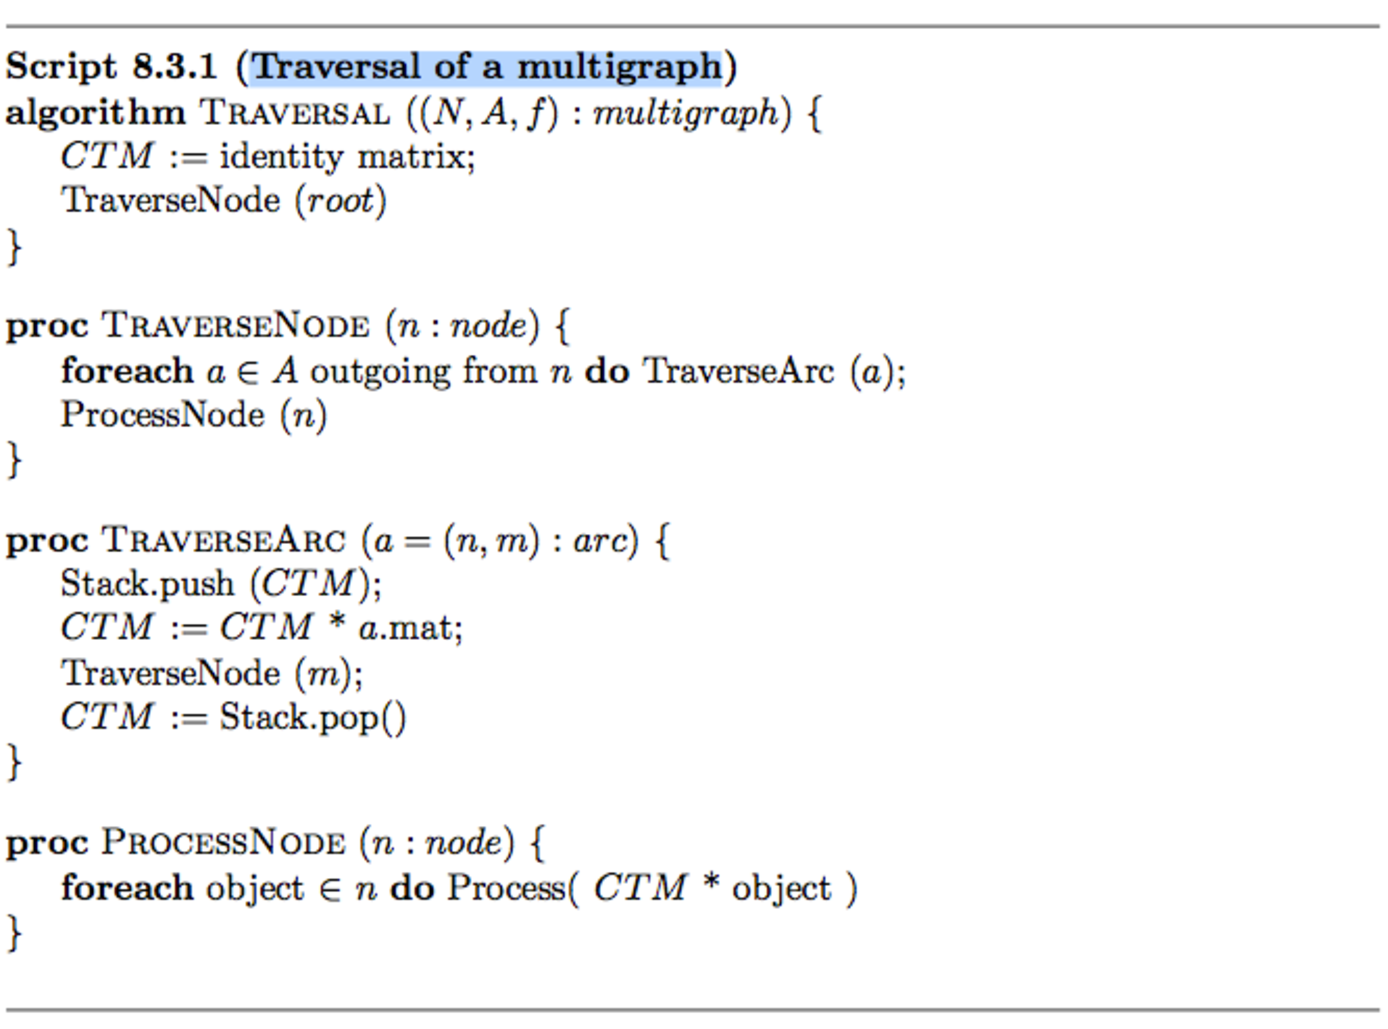
\includegraphics[width=0.8\linewidth]{images/traversal} 
   \caption{Traversal algorithm of a multigraph.}
   \label{fig:example}
\end{figure}


\subsubsection{Traversal of nested lists}

\paragraph{show the pattern of calls and returned values}

%-------------------------------------------------------------------------------
\begin{flushleft} \small \label{scrap26}
\protect\makebox[0ex][r]{\NWtarget{nuweb11}{\rule{0ex}{0ex}}\hspace{1em}}$\langle\,$Traversal of a multigraph\nobreak\ {\footnotesize 11}$\,\rangle\equiv$
\vspace{-1ex}
\begin{list}{}{} \item
\mbox{}\verb@def traverse(CTM, stack, o, flag):@\\
\mbox{}\verb@    i = 0@\\
\mbox{}\verb@    while i < len(o):@\\
\mbox{}\verb@        #print "lunghezza lista", len(o)@\\
\mbox{}\verb@        if ISNUM(o[i]): print o[i], REVERSE(CTM)@\\
\mbox{}\verb@        if ISSTRING(o[i]): @\\
\mbox{}\verb@            #print "E' una lettera " + o[i]@\\
\mbox{}\verb@            CTM.append(o[i])@\\
\mbox{}\verb@            #print "trasformazione attuale", CTM@\\
\mbox{}\verb@            if flag: stack.append(o[i])@\\
\mbox{}\verb@        if ISLIST(o[i]):@\\
\mbox{}\verb@            stack = [] @\\
\mbox{}\verb@            #print "E' una sottolista", o[i]@\\
\mbox{}\verb@            traverse(CTM, stack, o[i], True)@\\
\mbox{}\verb@            CTM = CTM[:-len(stack)]@\\
\mbox{}\verb@            stack = []@\\
\mbox{}\verb@            flag = False@\\
\mbox{}\verb@        i = i + 1@\\
\mbox{}\verb@@\\
\mbox{}\verb@def algorithm(data):@\\
\mbox{}\verb@    CTM,stack = ["I"],[]@\\
\mbox{}\verb@    traverse(CTM, stack, data, False)  @\\
\mbox{}\verb@@{\NWsep}
\end{list}
\vspace{-1ex}
\footnotesize\addtolength{\baselineskip}{-1ex}
\begin{list}{}{\setlength{\itemsep}{-\parsep}\setlength{\itemindent}{-\leftmargin}}
\item {\NWtxtMacroNoRef}.
\end{list}
\end{flushleft}
%-------------------------------------------------------------------------------
  
%-------------------------------------------------------------------------------
\begin{flushleft} \small \label{scrap27}
\protect\makebox[0ex][r]{\NWtarget{nuweb12a}{\rule{0ex}{0ex}}\hspace{1em}}$\langle\,$Examples of multigraph traversal\nobreak\ {\footnotesize 12a}$\,\rangle\equiv$
\vspace{-1ex}
\begin{list}{}{} \item
\mbox{}\verb@data = [1,"A", 2, 3, "B", [4, "C", 5], [6,"D", "E", 7, 8], 9]  @\\
\mbox{}\verb@data = [1,"A", [2, 3, "B", 4, "C", 5, 6,"D"], "E", 7, 8, 9]  @\\
\mbox{}\verb@data = [2, 3, "B", 4, "C", 5, 6,"D"]@\\
\mbox{}\verb@data = [1,"A", dat, "E", 7, 8, 9]@\\
\mbox{}\verb@@{\NWsep}
\end{list}
\vspace{-1ex}
\footnotesize\addtolength{\baselineskip}{-1ex}
\begin{list}{}{\setlength{\itemsep}{-\parsep}\setlength{\itemindent}{-\leftmargin}}
\item {\NWtxtMacroNoRef}.
\end{list}
\end{flushleft}
%-------------------------------------------------------------------------------


\paragraph{show the pattern of calls and returned values}

%-------------------------------------------------------------------------------
\begin{flushleft} \small \label{scrap28}
\protect\makebox[0ex][r]{\NWtarget{nuweb12b}{\rule{0ex}{0ex}}\hspace{1em}}$\langle\,$Let us explore the pattern even better\nobreak\ {\footnotesize 12b}$\,\rangle\equiv$
\vspace{-1ex}
\begin{list}{}{} \item
\mbox{}\verb@@\\
\mbox{}\verb@data = [@\\
\mbox{}\verb@   (1,6,@\\
\mbox{}\verb@      (7,1,@\\
\mbox{}\verb@         (8,"12"))),@\\
\mbox{}\verb@   (2,9,10),@\\
\mbox{}\verb@   (3,),@\\
\mbox{}\verb@   4,@\\
\mbox{}\verb@   (5,@\\
\mbox{}\verb@      (11,@\\
\mbox{}\verb@      ("13",)))]@\\
\mbox{}\verb@@\\
\mbox{}\verb@@\\
\mbox{}\verb@print list(traverse(data))@\\
\mbox{}\verb@@{\NWsep}
\end{list}
\vspace{-1ex}
\footnotesize\addtolength{\baselineskip}{-1ex}
\begin{list}{}{\setlength{\itemsep}{-\parsep}\setlength{\itemindent}{-\leftmargin}}
\item {\NWtxtMacroNoRef}.
\end{list}
\end{flushleft}
%-------------------------------------------------------------------------------

%-------------------------------------------------------------------------------
\subsection{aaaaaa}
%-------------------------------------------------------------------------------
%-------------------------------------------------------------------------------
\subsection{aaaaaa}
%-------------------------------------------------------------------------------
%===============================================================================
\section{Exporting the library}
%===============================================================================
%-------------------------------------------------------------------------------
\begin{flushleft} \small \label{scrap29}
\protect\makebox[0ex][r]{\NWtarget{nuweb13a}{\rule{0ex}{0ex}}\hspace{1em}}\verb@"lib/py/mapper.py"@\nobreak\ {\footnotesize 13a }$\equiv$
\vspace{-1ex}
\begin{list}{}{} \item
\mbox{}\verb@""" Mapping functions and primitive objects """@\\
\mbox{}\verb@@\hbox{$\langle\,$Initial import of modules\nobreak\ {\footnotesize \NWlink{nuweb15a}{15a}}$\,\rangle$}\verb@@\\
\mbox{}\verb@@\hbox{$\langle\,$Generate a simplicial decomposition ot the $[0,1]^d$ domain\nobreak\ {\footnotesize \NWlink{nuweb1}{1}}$\,\rangle$}\verb@@\\
\mbox{}\verb@@\hbox{$\langle\,$Create a dictionary with key the point location\nobreak\ {\footnotesize \NWlink{nuweb2b}{2b}}$\,\rangle$}\verb@@\\
\mbox{}\verb@@\hbox{$\langle\,$Primitive mapping function\nobreak\ {\footnotesize \NWlink{nuweb2a}{2a}}$\,\rangle$}\verb@@\\
\mbox{}\verb@@\hbox{$\langle\,$Basic tests of mapper module\nobreak\ {\footnotesize \NWlink{nuweb14b}{14b}}$\,\rangle$}\verb@@\\
\mbox{}\verb@@\hbox{$\langle\,$Circle centered in the origin\nobreak\ {\footnotesize \NWlink{nuweb3c}{3c}}$\,\rangle$}\verb@@\\
\mbox{}\verb@@\hbox{$\langle\,$Disk centered in the origin\nobreak\ {\footnotesize \NWlink{nuweb3d}{3d}}$\,\rangle$}\verb@@\\
\mbox{}\verb@@\hbox{$\langle\,$Ring centered in the origin\nobreak\ {\footnotesize \NWlink{nuweb4a}{4a}}$\,\rangle$}\verb@@\\
\mbox{}\verb@@\hbox{$\langle\,$Spherical surface of given radius\nobreak\ {\footnotesize \NWlink{nuweb5a}{5a}}$\,\rangle$}\verb@@\\
\mbox{}\verb@@\hbox{$\langle\,$Cylinder surface with $z$ axis\nobreak\ {\footnotesize \NWlink{nuweb4b}{4b}}$\,\rangle$}\verb@@\\
\mbox{}\verb@@\hbox{$\langle\,$Toroidal surface of given radiuses\nobreak\ {\footnotesize \NWlink{nuweb5b}{5b}}$\,\rangle$}\verb@@\\
\mbox{}\verb@@\hbox{$\langle\,$Half-toroidal surface of given radiuses\nobreak\ {\footnotesize \NWlink{nuweb6a}{6a}}$\,\rangle$}\verb@@\\
\mbox{}\verb@@\hbox{$\langle\,$Solid Sphere of given radius\nobreak\ {\footnotesize \NWlink{nuweb6b}{6b}}$\,\rangle$}\verb@@\\
\mbox{}\verb@@\hbox{$\langle\,$Solid cylinder of given radius and height\nobreak\ {\footnotesize \NWlink{nuweb6c}{6c}}$\,\rangle$}\verb@@\\
\mbox{}\verb@@\hbox{$\langle\,$Solid torus of given radiuses\nobreak\ {\footnotesize \NWlink{nuweb7a}{7a}}$\,\rangle$}\verb@@\\
\mbox{}\verb@@\hbox{$\langle\,$Solid pizza of given radiuses\nobreak\ {\footnotesize \NWlink{nuweb7b}{7b}}$\,\rangle$}\verb@@\\
\mbox{}\verb@@\hbox{$\langle\,$types Mat and Verts\nobreak\ {\footnotesize \NWlink{nuweb8b}{8b}}$\,\rangle$}\verb@@\\
\mbox{}\verb@@\hbox{$\langle\,$Translation matrices\nobreak\ {\footnotesize \NWlink{nuweb8c}{8c}}$\,\rangle$}\verb@@\\
\mbox{}\verb@@\hbox{$\langle\,$Scaling matrices\nobreak\ {\footnotesize \NWlink{nuweb9a}{9a}}$\,\rangle$}\verb@@\\
\mbox{}\verb@@\hbox{$\langle\,$Rotation matrices\nobreak\ {\footnotesize \NWlink{nuweb9b}{9b}}$\,\rangle$}\verb@@\\
\mbox{}\verb@@\hbox{$\langle\,$Embedding and projecting a geometric model\nobreak\ {\footnotesize \NWlink{nuweb3a}{3a}}$\,\rangle$}\verb@@\\
\mbox{}\verb@@\hbox{$\langle\,$Apply an affine transformation to a LAR model\nobreak\ {\footnotesize \NWlink{nuweb8a}{8a}}$\,\rangle$}\verb@@\\
\mbox{}\verb@@{\NWsep}
\end{list}
\vspace{-2ex}
\end{flushleft}
%-------------------------------------------------------------------------------
%===============================================================================
\section{Examples}
%===============================================================================

\paragraph{3D rotation about a general axis}

%-------------------------------------------------------------------------------
\begin{flushleft} \small \label{scrap30}
\protect\makebox[0ex][r]{\NWtarget{nuweb13b}{\rule{0ex}{0ex}}\hspace{1em}}\verb@"test/py/mapper/test02.py"@\nobreak\ {\footnotesize 13b }$\equiv$
\vspace{-1ex}
\begin{list}{}{} \item
\mbox{}\verb@""" General 3D rotation of a toroidal surface """@\\
\mbox{}\verb@@\hbox{$\langle\,$Initial import of modules\nobreak\ {\footnotesize \NWlink{nuweb15a}{15a}}$\,\rangle$}\verb@@\\
\mbox{}\verb@from mapper import *@\\
\mbox{}\verb@model = checkModel(larToroidal([0.2,1])())@\\
\mbox{}\verb@a,b,c = SCALARVECTPROD([PI/2,UNITVECT([1,1,0]) ])@\\
\mbox{}\verb@model = larApply(r(a,b,c))(model)@\\
\mbox{}\verb@VIEW(STRUCT(MKPOLS(model)))@\\
\mbox{}\verb@@{\NWsep}
\end{list}
\vspace{-2ex}
\end{flushleft}
%-------------------------------------------------------------------------------


\paragraph{3D rotation of a 2D circle}

%-------------------------------------------------------------------------------
\begin{flushleft} \small \label{scrap31}
\protect\makebox[0ex][r]{\NWtarget{nuweb14a}{\rule{0ex}{0ex}}\hspace{1em}}\verb@"test/py/mapper/test03.py"@\nobreak\ {\footnotesize 14a }$\equiv$
\vspace{-1ex}
\begin{list}{}{} \item
\mbox{}\verb@""" Elementary 3D rotation of a 2D circle """@\\
\mbox{}\verb@@\hbox{$\langle\,$Initial import of modules\nobreak\ {\footnotesize \NWlink{nuweb15a}{15a}}$\,\rangle$}\verb@@\\
\mbox{}\verb@from mapper import *@\\
\mbox{}\verb@model = checkModel(larCircle(1)())@\\
\mbox{}\verb@model = larEmbed(1)(model)@\\
\mbox{}\verb@model = larApply(r(PI/2,0,0))(model)@\\
\mbox{}\verb@VIEW(STRUCT(MKPOLS(model)))@\\
\mbox{}\verb@@{\NWsep}
\end{list}
\vspace{-2ex}
\end{flushleft}
%-------------------------------------------------------------------------------




%===============================================================================
\section{Tests}
%===============================================================================

	
%-------------------------------------------------------------------------------
\begin{flushleft} \small \label{scrap32}
\protect\makebox[0ex][r]{\NWtarget{nuweb14b}{\rule{0ex}{0ex}}\hspace{1em}}$\langle\,$Basic tests of mapper module\nobreak\ {\footnotesize 14b}$\,\rangle\equiv$
\vspace{-1ex}
\begin{list}{}{} \item
\mbox{}\verb@if __name__=="__main__":@\\
\mbox{}\verb@   V,EV = larDomain([5])@\\
\mbox{}\verb@   VIEW(EXPLODE(1.5,1.5,1.5)(MKPOLS((V,EV))))@\\
\mbox{}\verb@   V,EV = larIntervals([24])([2*PI])@\\
\mbox{}\verb@   VIEW(EXPLODE(1.5,1.5,1.5)(MKPOLS((V,EV))))@\\
\mbox{}\verb@      @\\
\mbox{}\verb@   V,FV = larDomain([5,3])@\\
\mbox{}\verb@   VIEW(EXPLODE(1.5,1.5,1.5)(MKPOLS((V,FV))))@\\
\mbox{}\verb@   V,FV = larIntervals([36,3])([2*PI,1.])@\\
\mbox{}\verb@   VIEW(EXPLODE(1.5,1.5,1.5)(MKPOLS((V,FV))))@\\
\mbox{}\verb@      @\\
\mbox{}\verb@   V,CV = larDomain([5,3,1])@\\
\mbox{}\verb@   VIEW(EXPLODE(1.5,1.5,1.5)(MKPOLS((V,CV))))@\\
\mbox{}\verb@   V,CV = larIntervals([36,2,3])([2*PI,1.,1.])@\\
\mbox{}\verb@   VIEW(EXPLODE(1.5,1.5,1.5)(MKPOLS((V,CV))))@\\
\mbox{}\verb@@{\NWsep}
\end{list}
\vspace{-1ex}
\footnotesize\addtolength{\baselineskip}{-1ex}
\begin{list}{}{\setlength{\itemsep}{-\parsep}\setlength{\itemindent}{-\leftmargin}}
\item \NWtxtMacroRefIn\ \NWlink{nuweb13a}{13a}.
\end{list}
\end{flushleft}
%-------------------------------------------------------------------------------

\paragraph{Circumference of unit radius}

%-------------------------------------------------------------------------------
\begin{flushleft} \small \label{scrap33}
\protect\makebox[0ex][r]{\NWtarget{nuweb14c}{\rule{0ex}{0ex}}\hspace{1em}}\verb@"test/py/mapper/test01.py"@\nobreak\ {\footnotesize 14c }$\equiv$
\vspace{-1ex}
\begin{list}{}{} \item
\mbox{}\verb@""" Circumference of unit radius """@\\
\mbox{}\verb@@\hbox{$\langle\,$Initial import of modules\nobreak\ {\footnotesize \NWlink{nuweb15a}{15a}}$\,\rangle$}\verb@@\\
\mbox{}\verb@from mapper import *@\\
\mbox{}\verb@model = checkModel(larCircle(1)())@\\
\mbox{}\verb@VIEW(EXPLODE(1.2,1.2,1.2)(MKPOLS(model)))@\\
\mbox{}\verb@"""@\\
\mbox{}\verb@model = checkModel(larDisk(1)([36,4]))@\\
\mbox{}\verb@VIEW(EXPLODE(1.2,1.2,1.2)(MKPOLS(model)))@\\
\mbox{}\verb@model = checkModel(larRing([.9, 1.])([36,2]))@\\
\mbox{}\verb@VIEW(EXPLODE(1.2,1.2,1.2)(MKPOLS(model)))@\\
\mbox{}\verb@model = checkModel(larCylinder([.5,2.])([32,1]))@\\
\mbox{}\verb@VIEW(STRUCT(MKPOLS(model)))@\\
\mbox{}\verb@model = checkModel(larSphere(1)())@\\
\mbox{}\verb@VIEW(STRUCT(MKPOLS(model)))@\\
\mbox{}\verb@model = larBall(1)()@\\
\mbox{}\verb@VIEW(STRUCT(MKPOLS(model)))@\\
\mbox{}\verb@model = larRod([.25,2.])([32,1])@\\
\mbox{}\verb@VIEW(STRUCT(MKPOLS(model)))@\\
\mbox{}\verb@model = checkModel(larToroidal([0.5,1])())@\\
\mbox{}\verb@VIEW(STRUCT(MKPOLS(model)))@\\
\mbox{}\verb@model = checkModel(larCrown([0.125,1])([8,48]))@\\
\mbox{}\verb@VIEW(STRUCT(MKPOLS(model)))@\\
\mbox{}\verb@model = larPizza([0.05,1])([8,48])@\\
\mbox{}\verb@VIEW(STRUCT(MKPOLS(model)))@\\
\mbox{}\verb@model = checkModel(larTorus([0.5,1])())@\\
\mbox{}\verb@VIEW(STRUCT(MKPOLS(model)))@\\
\mbox{}\verb@"""@\\
\mbox{}\verb@@{\NWsep}
\end{list}
\vspace{-2ex}
\end{flushleft}
%-------------------------------------------------------------------------------


%===============================================================================
\appendix
\section{Utility functions}
%===============================================================================

%-------------------------------------------------------------------------------
\begin{flushleft} \small \label{scrap34}
\protect\makebox[0ex][r]{\NWtarget{nuweb15a}{\rule{0ex}{0ex}}\hspace{1em}}$\langle\,$Initial import of modules\nobreak\ {\footnotesize 15a}$\,\rangle\equiv$
\vspace{-1ex}
\begin{list}{}{} \item
\mbox{}\verb@from pyplasm import *@\\
\mbox{}\verb@from scipy import *@\\
\mbox{}\verb@import os,sys@\\
\mbox{}\verb@@\\
\mbox{}\verb@""" import modules from larcc/lib """@\\
\mbox{}\verb@sys.path.insert(0, 'lib/py/')@\\
\mbox{}\verb@@\hbox{$\langle\,$Import the module\nobreak\ ({\footnotesize \NWtarget{nuweb15b}{15b}\label{scrap35}
 }\mbox{}\verb@lar2psm@ ) {\footnotesize \NWlink{nuweb16a}{16a}}$\,\rangle$}\verb@@\\
\mbox{}\verb@@\hbox{$\langle\,$Import the module\nobreak\ ({\footnotesize \NWtarget{nuweb15c}{15c}\label{scrap36}
 }\mbox{}\verb@simplexn@ ) {\footnotesize \NWlink{nuweb16a}{16a}}$\,\rangle$}\verb@@\\
\mbox{}\verb@@\hbox{$\langle\,$Import the module\nobreak\ ({\footnotesize \NWtarget{nuweb15d}{15d}\label{scrap37}
 }\mbox{}\verb@larcc@ ) {\footnotesize \NWlink{nuweb16a}{16a}}$\,\rangle$}\verb@@\\
\mbox{}\verb@@\hbox{$\langle\,$Import the module\nobreak\ ({\footnotesize \NWtarget{nuweb15e}{15e}\label{scrap38}
 }\mbox{}\verb@largrid@ ) {\footnotesize \NWlink{nuweb16a}{16a}}$\,\rangle$}\verb@@\\
\mbox{}\verb@@\hbox{$\langle\,$Import the module\nobreak\ ({\footnotesize \NWtarget{nuweb15f}{15f}\label{scrap39}
 }\mbox{}\verb@boolean2@ ) {\footnotesize \NWlink{nuweb16a}{16a}}$\,\rangle$}\verb@@\\
\mbox{}\verb@@{\NWsep}
\end{list}
\vspace{-1ex}
\footnotesize\addtolength{\baselineskip}{-1ex}
\begin{list}{}{\setlength{\itemsep}{-\parsep}\setlength{\itemindent}{-\leftmargin}}
\item \NWtxtMacroRefIn\ \NWlink{nuweb13a}{13a}\NWlink{nuweb13b}{b}\NWlink{nuweb14a}{, 14a}\NWlink{nuweb14c}{c}.
\end{list}
\end{flushleft}
%-------------------------------------------------------------------------------

%-------------------------------------------------------------------------------
\begin{flushleft} \small \label{scrap40}
\protect\makebox[0ex][r]{\NWtarget{nuweb16a}{\rule{0ex}{0ex}}\hspace{1em}}$\langle\,$Import the module\nobreak\ {\footnotesize 16a}$\,\rangle\equiv$
\vspace{-1ex}
\begin{list}{}{} \item
\mbox{}\verb@import @@1\verb@@\\
\mbox{}\verb@from @@1\verb@ import *@\\
\mbox{}\verb@@{\NWsep}
\end{list}
\vspace{-1ex}
\footnotesize\addtolength{\baselineskip}{-1ex}
\begin{list}{}{\setlength{\itemsep}{-\parsep}\setlength{\itemindent}{-\leftmargin}}
\item \NWtxtMacroRefIn\ \NWlink{nuweb15a}{15a}.
\end{list}
\end{flushleft}
%-------------------------------------------------------------------------------


\subsection{Numeric utilities}

A small set of utilityy functions is used to transform a point representation as array of coordinates into a string of fixed format to be used as point key into python dictionaries.

%------------------------------------------------------------------
\begin{flushleft} \small \label{scrap41}
\protect\makebox[0ex][r]{\NWtarget{nuweb16b}{\rule{0ex}{0ex}}\hspace{1em}}$\langle\,$Symbolic utility to represent points as strings\nobreak\ {\footnotesize 16b}$\,\rangle\equiv$
\vspace{-1ex}
\begin{list}{}{} \item
\mbox{}\verb@""" TODO: use package Decimal (http://docs.python.org/2/library/decimal.html) """@\\
\mbox{}\verb@ROUND_ZERO = 1E-07@\\
\mbox{}\verb@def round_or_zero (x,prec=7):@\\
\mbox{}\verb@   """@\\
\mbox{}\verb@   Decision procedure to approximate a small number to zero.@\\
\mbox{}\verb@   Return either the input number or zero.@\\
\mbox{}\verb@   """@\\
\mbox{}\verb@   def myround(x):@\\
\mbox{}\verb@      return eval(('%.'+str(prec)+'f') % round(x,prec))@\\
\mbox{}\verb@   xx = myround(x)@\\
\mbox{}\verb@   if abs(xx) < ROUND_ZERO: return 0.0@\\
\mbox{}\verb@   else: return xx@\\
\mbox{}\verb@@\\
\mbox{}\verb@def prepKey (args): return "["+", ".join(args)+"]"@\\
\mbox{}\verb@@\\
\mbox{}\verb@def fixedPrec(value):@\\
\mbox{}\verb@   if abs(value - int(value))<ROUND_ZERO: value = int(value)@\\
\mbox{}\verb@   out = ('%0.7f'% value).rstrip('0')@\\
\mbox{}\verb@   if out == '-0.': out = '0.'@\\
\mbox{}\verb@   return out@\\
\mbox{}\verb@   @\\
\mbox{}\verb@def vcode (vect): @\\
\mbox{}\verb@   """@\\
\mbox{}\verb@   To generate a string representation of a number array.@\\
\mbox{}\verb@   Used to generate the vertex keys in PointSet dictionary, and other similar operations.@\\
\mbox{}\verb@   """@\\
\mbox{}\verb@   return prepKey(AA(fixedPrec)(vect))@\\
\mbox{}\verb@@{\NWsep}
\end{list}
\vspace{-1ex}
\footnotesize\addtolength{\baselineskip}{-1ex}
\begin{list}{}{\setlength{\itemsep}{-\parsep}\setlength{\itemindent}{-\leftmargin}}
\item {\NWtxtMacroNoRef}.
\end{list}
\end{flushleft}
%------------------------------------------------------------------


\bibliographystyle{amsalpha}
\bibliography{mapper}

\end{document}
